\documentclass[conference]{IEEEtran}
\IEEEoverridecommandlockouts
% The preceding line is only needed to identify funding in the first footnote. If that is unneeded, please comment it out.
\usepackage{cite}
\usepackage{amsmath,amssymb,amsfonts}
\usepackage{algorithmic}
\usepackage{graphicx}
\usepackage{textcomp}
\usepackage{xcolor}
\usepackage{url}
\def\BibTeX{{\rm B\kern-.05em{\sc i\kern-.025em b}\kern-.08em
    T\kern-.1667em\lower.7ex\hbox{E}\kern-.125emX}}
\begin{document}

\title{The Decision Making of Self-driving Vehicles: A Survey}

\author{\IEEEauthorblockN{1\textsuperscript{st} Wenxing Lan}
\IEEEauthorblockA{\textit{dept. name of organization (of Aff.)} \\
\textit{name of organization (of Aff.)}\\
City, Country \\
email address or ORCID}


}

\maketitle

\begin{abstract}

\end{abstract}

\begin{IEEEkeywords}
component, formatting, style, styling, insert
\end{IEEEkeywords}

\section{Introduction}
Autonomous vehicles (also known as self-driving vehicles and driverless vehicles) have been researched by many universities, research institutes, internet companies, vehicle companies and companies of other industries around the world since the middle 1980s~\cite{self_driving}. In the last two decades, several crucial of autonomous vehicle research platforms are as follows: the Navlab's mobile platform~\cite{Thorpe199144}, University of Pavia's and Parma's car, ARGO~\cite{Broggi199955}, and UBM's vehicles, VaMoRs and VaMP~\cite{Gregor200248}.

In the last decade, the Defence Advanced Research Projects Agency (DARPA) organized three competitions to accelerate the development of correlation technique about autonomous vehicles~\cite{Brian2016}. In 2004, the first competition named as DARPA Grand Challenge was held in the Mojave Desert, USA~\cite{self_driving}. The goal is to get autonomous vehicles to travel 140 miles of off-road routes as fast as possible~\cite{Brian2016}. Unfortunately, there is no autonomous vehicle which was able to complete the whole journey~\cite{self_driving}.

In 2005, the DARPA Grand Challenge was held again and required autonomous vehicles to travel 132 miles of difficult desert roads across Nevada which contain a mixture of featureless terrain, dust, global positioning system drop-outs, sharp turns, narrow openings, bridges, railroad overpasses, long tunnels, obstacles and a narrow winding mountains road with a 200-foot drop-off~\cite{Buehler2007}. This competition had 23 finalists and 4 cars finished the course within 10-hour limit. Remarkably, the Stanford University's vehicles, Stanley, won the first-place prize, and the Carnegie Mellon University's cars, Sandstorm and H1ghlander, came in second and third place, respectively~\cite{Buehler2007}.

The third competition which is named as the DARPA Urban Challenge was held at the now-closed George Air Force Base, California, USA, in 2007. The objective was for a autonomous vehicles to complete the 60 mile course in less than 6 hours. Additionally, the autonomous vehicles were asked to obey all traffic regulations which avoiding other vehicles including driverless and humandriven vehicles~\cite{buehler2009darpa}. There are 11 finalists in this competition and 6 vehicles completed the route within the allotted time limit. Specifically, Boss, the vehicle of Carnegie Mellon University, won the first-place prize, the Stanford University's car, Junior, claimed second place, and the Virginia Tech's car, Odin, finished in third~\cite{buehler2009darpa}. Although the challenges presented by these competitions cannot cover all the challenges encountered in everyday traffic, they have been hailed as milestones in the development of autonomous vehicles~\cite{Brian2016}.

After the DARPA Challenge, there was a flood of driverless events. Relevant examples include: Intelligent Vehicle Future Challenges~\cite{xin2014china}, from 2009 to 2013; Hyundai Autonomous Challenge~\cite{Cerri2011}, which was held in 2010; VisLab Intercontinental Autonomous Challenge~\cite{broggi2012vislab}, in 2010; the Grand Cooperative Driving Challenge (GCDC)~\cite{Englund2016}, in 2011 and 2016 and Public Road Urban Driverless-Car Test~\cite{Broggi2015}, which was held in 2013. At the same time, many industrial and academic teams have invested a lot of research and development energy in the field of autonomous driving. Among them, the industry is represented by the OEMs of Ford, Toyota, Hyundai and other car companies, as well as IT and emerging companies such as Waymo, Tesla, Uber, Intel, Baidu, Pony.ai, etc., and have developed various autonomous vehicle platforms based on commercialization goals; Academia, including CMU, Stanford, UC Berkeley, Tsinghua University, Tongji University, Southern University of Science and Technology and other major domestic and foreign universities have carried out a series of researches around the key technical fields of autonomous driving.

In order to regulate the application of unmanned driving technology, the National Highway Transportation Safety Administration of the United States Department of Transportation has divided the level of automatic driving (based on the SAE International Standard J3016~\cite{sae2018taxonomy}):
\begin{enumerate}
	\item Level 0 (manual driving): completely controlled by a human driver;
	\item Level 1 (assisted driving): The driving environment provides support for one of the steering wheel and acceleration and deceleration operations, and the rest is operated by humans. Contains basic auxiliary driving, such as adaptive cruise control (ACC), anti-lock brake system (ABS), electronic stability control system (ESC);
	\item Level 2 (semi-automatic driving): The driving environment provides support for multiple operations in the steering wheel and acceleration and deceleration, and the rest is operated by humans.  Contains some advanced auxiliary driving functions, such as a horizontal/vertical control system with minimal risk, emergency braking, etc.;
	\item Level 3 (Highly Autonomous Driving): The unmanned driving system completes all operations, but requires the human driver to take over when leaving the operational scene of unmanned driving.
	\item Level 4 (Ultra-high auto-driving): An unmanned driving system with limited roads and environmental conditions, and does not require human drivers to respond to system requests.
	\item Level 5 (Fully Automated Driving): Unmanned driving system that does not limit roads and environmental conditions
\end{enumerate}

The perception system and the decision-making system are two main parts of the autonomy system architecture of autonomous vehicle~\cite{Brian2016}. To limit the scope of this survey, We focus on some aspects of decision-making system, which includes route planning, path planning, behavior selection, motion planning, obstacle avoidance and control, in particular, for systems falling into the automation level of 3 and above~\cite{self_driving}.
The remainder of the paper id structured as follows:
\begin{enumerate}
	\item Overview of the Decision-Making Hierarchy
	\item Route planning
	\item Path planning
	\item Behavior selector
	\item Motion planning
	\item Obstacle Avoidance and control
	\item Conclusion
\end{enumerate}


\section{Overview of the Decision-Making Hierarchy}

\begin{figure}[htbp]
	\centering
	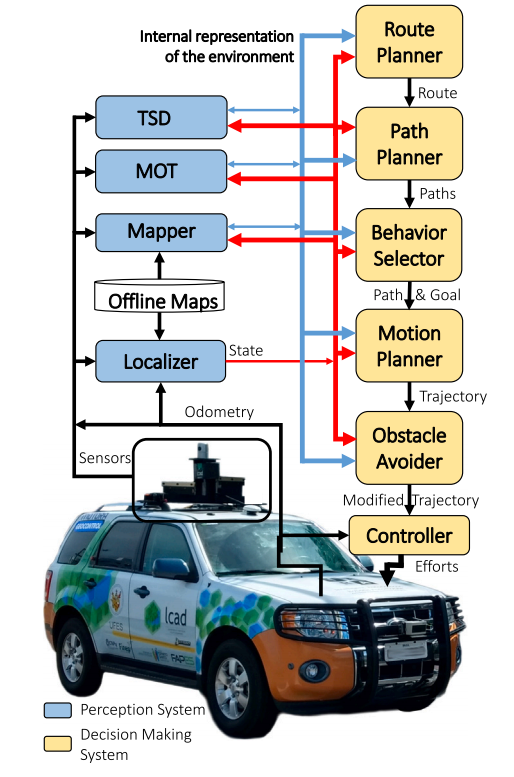
\includegraphics[width=1\columnwidth]{./picture/architecture.png}
	\caption{\label{architecture}
		The five subsystems of decision making system of a typical autonomous vehicle.}
\end{figure}

In this section, the decision making system of a typical autonomous vehicles is described and the brief description of each component of decision making system is provided. The perception system of autonomous vehicles use data captured by on-board sensors, such as Light Detection and Ranging (LIDAR), Radio Detection and Ranging (RADAR), camera, Global Positioning System (GPS), Inertial Measurement Unit (IMU), odometer, etc., and prior information about the models of sensors, road network, traffic rules, vehicle dynamics, etc. to estimate the state of vehicles and create representation of the surrounding environment~\cite{self_driving}. Then, the decision making system use the estimation and environment constructed to control the vehicle in order to reach the goal object~\cite{Brian2016}. 

There are six subsystems which are shown as the orange blocks in Fig~\ref{architecture} in the decision making system of a typical autonomous vehicles~\cite{self_driving}. The brief description of each subsystem is shown as belows.

\subsection{Route Planning Subsystem}
Given a requested destination defined in the road network by the user, the route planning subsystem aims to compute a route, $R$, through the road network from its current position to the requested destination~\cite{Brian2016}. A route, $R=\{r_1, r_2,...,r_{|R|}\}$, is a sequence of way point, where each way point, $r_i$ where $i \in \{1,2,...,|R|\}$, is a coordinate pair. i.e. $r_i = (x_i, y_i)$, in the road network~\cite{self_driving}. Actually, route palnning is a kind of global route planning since it needs to find the complete route from ego vehicle's current position to the final goal, such as the route planned by the BAIDU maps\footnote{https://map.baidu.com/}. The related methods for route planning is shown is Section~\ref{sec:route_planner}.

\subsection{Path Planning Subsystem}
Given a route computed by the route planning subsystem, the path planning subsystem computes a set of paths, $P=\{P_1, P_2, ..., P_{|P|}\}$ by considering the ego vehicle's current state and the traffic rules as well as the surrounding environment~\cite{self_driving}. A path is a sequence of poses, i.e. $P_j=\{p_1, p_2, ..., p_{|P_j|}\}$ where $j \in \{1, 2,...,|P|\}$~\cite{self_driving}. Additionally, each pose, $p_i$, is a coordinate tuple in the static map which only has static object, such as static obstacles, buildings and roads, aroung the ego vehicle and the desired vehicle's orientation at the position defined by this tuple, i.e., $p_i=(x_i, y_i, \theta_i)$~\cite{self_driving}. The relevant methods used in path planning subsystem will be given in Section~\ref{sec:path_planner}.

\subsection{Behavior Selection Subsystem}
The behavior selection subsystem is responsible to select the current reasonable driving behavior for the vehicle according to the behavior, traffic rules and road conditions of the current surrounding traffic participants~\cite{Brian2016}. The behaviors output here are specific driving maneuvers, such as acceleration and deceleration, lane change, overtaking, and following~\cite{Brian2016}. Additionally, the behavior selection subsystem need to select a pose in a selecting path among a set of paths generated by path palnning subsystem a few seconds ahead of the current ego vehicle's state~\cite{self_driving}. The relevant methods used in Path Behavior Selector is shown in Section~\ref{sec:behavior_selector}.

\subsection{Motion Planning Subsystem}
When the behavior is selected by the behavior selection subsystem (for example, it may be lane changing or left turning), motion planning subsystem needs to find a trajectory $T$ which is form the current ego vehicle's state to the curent goal state~\cite{Brian2016}. More importantly, the trajectory needs to satisfy the kinematic and dynamic constraints and be confortable for passengers~\cite{self_driving}. The trajectory $T=\{c_1, c_2, ..., c_{|T|}\}$ can be defined as a sequence of commands, $c_k=(v_k, \phi_k, \Delta_{t_k})$, where $v_k$ denotes the desired velocity at time $k$, $\phi_k$ represents the desired steering angle at time $k$, and $\Delta_{t_k}$ is the duration of $c_k$~\cite{self_driving}. In Section~\ref{sec:motion_planner}, the detail of methods used in motion planning subsystem will be given.

\subsection{Obstacle Avoidance Subsystem}
The obstacle avoidance subsytem needs to change the trajectory (usually decreasing the speed) which is the output of motion planning subsystem in order to avoid collision with other obstacle~\cite{self_driving}.  There is little literature on how to perform the function of this subsystem. Some of the literature related to this subsystem will be discussed in Section~\ref{sec:obstacle_avoider}.


\section{Related Work of Route Planning Subsystem}\label{sec:route_planner}
In this section, the related techniques reported in the literature for the Route Planner subsystem will be surveyed.

The road network, which is the input of the route planning subsystem, is usually represented as a weighted directed graph $G=(V, E)$~\cite{self_driving}. In weighted directed graph $G$, each vertex $v_i$ where $v_i \in V=\{v_1, v_2, ..., v_{|V|}\}$ is road junction, such as crossroads, three forks, etc., and each directed edge $e_{ij}$ where $e_{i,j} \in E, i \neq j$ connects pairs of road junctions $v_i$ and $v_j$. Specifically, edge weight $w_{ij}$ denotes the cost of traversing edge $e_{ij}$. Computing a route, the task of route planning subsystem, can be reduced to find a path in a weighted directed graph. Normally, the path should be shorest since most users are willing to reach destination as soon as possible~\cite{self_driving}. Unfortunately, classical shortest path algorithms, such as Dijkstra~\cite{dijkstra1959note} and $A^*$~\cite{Hart1968formal} are impractical because of their high time complexity to large road networks, such as city road network or even nation road network~\cite{self_driving}.


\section{Related Work of Path Planning Subsystem}\label{sec:path_planner}
\section{Related Work of Behavior Selection Subsystem}\label{sec:behavior_selector}
\section{Related Work of Motion Planning Subsystem}\label{sec:motion_planner}
\section{Related Work of Obstacle Avoidance Subsystem}\label{sec:obstacle_avoider}
\section{Conclusion}


\section*{Acknowledgment}


\bibliographystyle{IEEEtran}
\bibliography{decision_making} 

\end{document}

